\section{Frame design and construction}
The 2009 frame design underwent a complete revision based on our
experience from previous years.  Our past frame designs included
custom ordered molded or rapid prototyped parts intended to improve
the hydrodynamics of the hull.  After analyzing the conditions that
the vehicle would be subjected to, it was determined that the effects
of fluid dynamics were negligible in terms of functionality.  For this
reason, a ``design for manufacturing'' development methodology was
adopted: in efforts to minimize cost and machining time, the frame has been
designed to take advantage of commercial off-the-shelf parts as
well as capitalize on simple manufacturing processes.

\subsection{Design Considerations}
\label{fobjectives}
The design objectives in the 2009 frame were significantly more
ambitious as our team included more members adept in manufacturing.
The final concept was conceived such that it could be fabricated
without the need for outsourcing.

Below is the list of the desirable attributes for the frame that we set out to
obtain based on the experience gained from past frame designs:
\begin{packed_enum}
\item Minimize time required to access batteries and electronics;
\item Maximize modularity for easier transport and progressive revisions;
\item Optimize mass for transport, functionality and points;
\item Provide a secure removable internal rack for electronics to facilitate bench testing;
\item Obtain a a waterproof seal with a simple low tolerance assembly;
\item Create solid harness points and handles;
\item Facilitate movement through water and maximize battery life with
  a neutrally buoyant design;
\item Compensate for changes in mass distribution and motion
  calibration with adjustable thruster positions;
\item Design an attractive and professional looking vehicle.
\end{packed_enum}

\subsection{Frame Overview}
The AquaTux frame design can be divided into three
subsections: external frame, hull, and internal rack.  The goals based
on past experience described above suggested the need to
minimize the number of sealing surfaces and reduce the number of
waterproof connectors.  To achieve these objectives, a single enclosure
was created (the hull) to encapsulate everything except for the
markers to be dropped, the thrusters and the hydrophones.  These external components would be
connected to an exoskeleton type frame which allows for flexible
mounting arrangements.  Finally an internal rack was designed to hold
 all the electrical components including cameras and embedded computer.

\subsubsection{External Frame}
The external frame was designed with transportation and fabrication as
the primary constraints. This exoskeleton is made entirely of
commercial off-the-shelf
parts, $\frac{1}{2}$ inch PVC plumbing pipe and connectors.  The thruster positions
are fully adjustable since they are attached to individual pipes fixed
in place by standard gear clamps (Figure~\ref{adj}). The adjustability of the frame also
facilitates transportation as the entire structure can be collapsed to
fit a smaller envelope. 

\begin{figure}
\begin{center}
 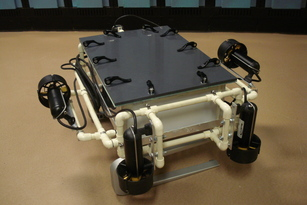
\includegraphics[width=3in]{fig/dsc06455} 
% 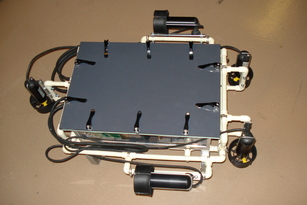
\includegraphics[width=3in]{fig/dsc06453} 
\vspace{.05in}
\hrule
\caption{Adjustable PVC tube exoskeleton frame.}\label{adj}
\end{center}
\end{figure}

In order to ensure a simple assembly method and utilize standard
connectors, the mechanism for picking up the briefcase was made of the
same material as the external frame.  It utilizes the fact that the
target is an open-walled structure and consists of a fork designed to
spear the case so that it can surface with the vehicle.

\subsubsection{Hull}
This year's hull design attempts to minimize the number of sealing
surfaces while maintaining usable space inside the vehicle.  In order
to seal the hull, a lid was made with a special simplified o-ring
groove (Figure~\ref{oring}). To avoid the need for precision milling or numerically
controlled machines, an oversized rectangular groove was cut.  The
corners were then drilled out and replaced with nylon dowels to
prevent the sharp corners from cutting into the o-ring.  This design
eliminated the need for specialized end mills or the need to mill
curved patterns in the lid. 

\begin{figure}
\begin{center}
 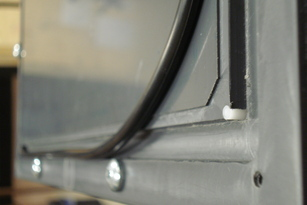
\includegraphics[width=3in]{fig/dsc06460.jpg} 
\vspace{.05in}
\hrule
\caption{O-ring displaced to show the grooves and nylon dowel.}\label{oring}
\end{center}
\end{figure}

Past experience suggested the need for a quicker method to access the
internal components of the hull.  Quick-release latches 
(Figure~\ref{quick}), were
used to replace nuts and bolts which take significantly more time to
release.  These latches use a cam mechanism to clamp the lid to
metallic bars and subsequently compress the o-ring, creating a water-tight seal.

\begin{figure}
\begin{center}
 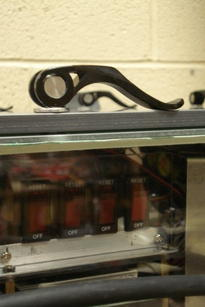
\includegraphics[width=1.34in]{fig/dsc06462} 
\vspace{.05in}
\hrule
\caption{Quick release cover mechanism.}\label{quick}
\end{center}
\end{figure}

An endplate was designed to provide a single replaceable surface to accept all the connectors between the interior and exterior of the vehicle.  This endplate is sealed with a groove similar to that of the lid and is attached with self sealing screws from APM Hexseal.  The waterproof connectors which pass through the endplate lead to two master-disconnects which allow for quick and easy installation of the internal rack (Figure~\ref{endplate}).
The waterproof connectors chosen are 8-pin Neoprene molded connectors
from Impulse Enterprise.  These connect the thrusters as well as the
wireless tether and provide maximal flexibility due to their pin count
as well as small profile.  
The pressure readings for the AUV are also gathered  through the
endplate. In order to sense depth, a MPX4115 pressure transducer is
coupled to a segment of PVC tubing connected to a compression nut on
the endplate.  The depth of the vehicle corresponds to the pressure of
the air trapped in the PVC tubing.
  The hull is fabricated from
$\frac{1}{8}$ inch thick polycarbonate sheets, with waterproof epoxy bonding
the joints together.  To strengthen the bonds, aluminum angle brackets
were added to the edges to increase the bonding area of the epoxy. The thin, clear polycarbonate walls of the hull allow subsystems such as the cameras, marker droppers (section~\ref{mdroppers}) and trigger for the torpedo to operate from within the vessel.

\begin{figure}
\begin{center}
\subfigure[Endplate showing waterproof connectors.]{ 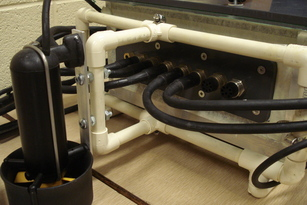
\includegraphics[width=3in]{fig/dsc06464} }
\subfigure[Master disconnects for the waterproof connectors on the
inside of the vehicle.]{ 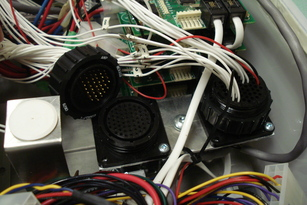
\includegraphics[width=3in]{fig/dsc06465} }
\vspace{.05in}
\hrule
\caption{Connection system to the outside of the vehicle.}\label{endplate}
\end{center}
\end{figure}

\subsubsection{Internal Rack}
In addition to remedying problems with our previous frames, we
endeavored to produce a frame that could be reconfigured and usable in
future years.  The concept for the internal rack (Figure~\ref{rack})
consists of base plates that accepts stacks of electronics.  These
plates can be removed as a single unit which facilitates wiring, and
bench testing.  Due to the buoyancy of the hull, stainless steel bars
were used to add weight to the vehicle (Figure~\ref{rack}).  These weights act as a method of balancing the
vessel and allow the electrical components to be reconfigured for
years to come.  The internal rack does not rest directly on the floor
of the hull.  In case of a leak, water would collect in the space
below the electrical components and be detected with leak sensors
prior to any damage.


\begin{figure}
\begin{center}
 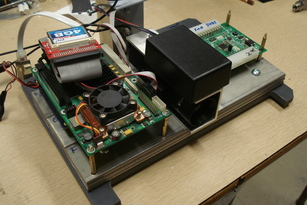
\includegraphics[width=3in]{fig/dsc06466} 
\vspace{.05in}
\hrule
\caption{Inside rack holding the electronics and the stainless steel weights.}\label{rack}
\end{center}
\end{figure}


\section{The Marker Dropper}
\label{mdroppers}

The thin walls of the hull facilitate the operation of a simple marker dropper system which
can be centered around the downward facing camera.  Two ferrous
markers are placed on the exterior of the vessel and held in place by
a magnetic attraction to two rare earth magnets located on the inside
of the hull.  The magnets are connected to individual stepper motors
which retract the magnets from the wall of the hull (Figure~\ref{md2}).  The increased
distance between the magnets and the markers causes a reduction in
magnetic field strength allowing the markers to drop freely from the
vehicle.

\begin{figure}
\begin{center}
 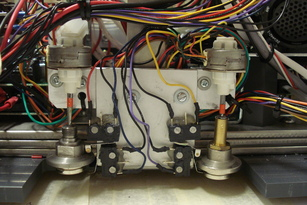
\includegraphics[width=3in]{fig/dsc06468} 
\vspace{.05in}
\hrule
\caption{Two marker-droppers: from top to bottom, a stepper motor
  retracts a magnet from the surface of the hull (bottom in the figure).}\label{md2}
\end{center}
\end{figure}

\section{The Torpedo Launcher}
\label{torpedo}
\vspace{-.1in}
One of the primary goals of this year's entry into the AUV Competition
was to minimize the number of connections that pass through the
endplate of the hull.  The resulting design for a torpedo launcher was
an external system that was activated by a magnetic switch.  This
concept allowed us to mimic the marker dropper design to activate the
torpedo.  The external system  contains only a few simple parts; a
power supply (9V battery), a solenoid valve, a magnetic switch, a
compressed gas cylinder and a projectile. As the magnet in the hull
is retracted from the hull, the magnetic switch is
triggered.  The switch  then triggers the solenoid valve allowing
compressed gas to fire the torpedo.

The controls for the above mentioned systems are described in the
following sections.
